\documentclass[12pt,a4paper]{article}
\usepackage[utf8]{inputenc}
\usepackage[catalan]{babel}
\usepackage{geometry}
\usepackage{fancyhdr}
\usepackage{tabularx}
\usepackage{lastpage}
\usepackage{enumitem}
\usepackage{amsmath}
\usepackage{amsfonts}
\usepackage{amssymb}
\usepackage{tikz}
\usepackage{pgfplots}
\usepackage[most]{tcolorbox} 
\usepackage{graphicx}
\pgfplotsset{compat=1.18}

% 1. MARGES I CAPÇALERA
\geometry{top=3cm, bottom=2.5cm, left=2cm, right=2cm, headheight=2.5cm}

\pagestyle{fancy}
\fancyhf{}
% Capçalera amb les teves imatges
\fancyhead[L]{
\includegraphics[height=1.8cm]{Logo_Departament.png}} 
\fancyhead[R]{
\includegraphics[height=1.8cm]{Logo_Institut.png}}

\fancyfoot[C]{Pàgina \thepage\ de \pageref{LastPage}}
\renewcommand{\headrulewidth}{0.4pt}

\begin{document}

% --- CAPÇALERA D'IDENTIFICACIÓ ---
\begingroup
\renewcommand{\arraystretch}{2.2}
\begin{tabularx}{\textwidth}{|X|p{4cm}|}
    \hline
    \textbf{Nom i cognoms:} & \textbf{Grup:} \\ \hline
    \textbf{Activitat:} Funcions lineals i afins & \textbf{Data:} \\ \hline
\end{tabularx}
\endgroup

\vspace{0.5cm}

\begin{center}
    {\Large \textbf{ACTIVITAT 2: FUNCIONS LINEALS I AFINS}}
\end{center}

% --- TEORIA (Text original del PDF) ---
\section*{Funcions Lineals}
Les funcions lineals descriuen relacions de \textbf{proporcionalitat directa} entre les variables. Són exemples de funcions lineals:
\begin{itemize}
    \item El cost total dels préssecs en funció del pes comprat si els préssecs costen \textbf{4 €/kg}.
    \[ f(x) = 4x \]
    \item El nombre de potes total dins un corral de gallines (2 potes per gallina).
    \[ f(x) = 2x \]
\end{itemize}
L'expressió algebraica de les funcions lineals té forma de $\boldsymbol{f(x)=mx}$ on $m \neq 0$.
\begin{tcolorbox}[colback=blue!5,colframe=blue!40, title=Recorda]
La seva representació gràfica sempre és una recta que passa pel punt \textbf{(0,0)}, que és l'origen de coordenades.
\end{tcolorbox}

\section*{Funcions Afins}
Les funcions afins descriuen situacions en què cal sumar un terme constant a un terme directament proporcional. Tenen la forma $\boldsymbol{f(x)=mx+n}$ on $m \neq 0$ i $n \neq 0$. Són exemples de funcions afins:
\begin{itemize}
    \item El cost d'un viatge de \textbf{taxi} que costa 6 € la baixada de bandera (només en començar el viatge) i 0,5 € el km.
    \[ f(x) = 0,5x + 6 \]
    \item El cost d'una factura de \textbf{gas} que costa 10 € de terme fix i 2 € per cada $m^3$ gastat.
    \[ f(x) = 2x + 10 \]
\end{itemize}
La seva representació gràfica és una recta que \textbf{no passa} per l'origen (0,0).
\begin{center}
    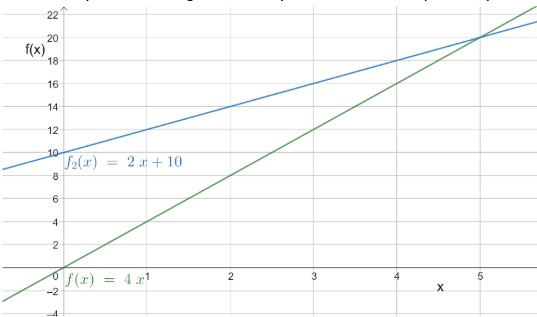
\includegraphics[]{AfiLineal.jpg} 
\end{center}
% --- EXERCICI 1 ---
\section*{1. Representació inicial}
Representa les següents funcions a la graella:
\textit{Pista:} Dona diferents valors a $x$ (negatius i positius), substitueix-los a la fórmula i calcula el resultat $f(x)$ o $g(x)$.

\vspace{0.5cm}

% --- BLOC DE CÀLCULS I TAULES ---
\noindent
\begin{minipage}[t]{0.48\textwidth}
    \textbf{1. Funció $f(x) = x + 1$} \\
    
    \textit{Càlculs:}
    \begin{itemize}
        \item $f(-2) = \dots\dots\dots\dots$
        \item $f(-1) = \dots\dots\dots\dots$
        \item $f(0) = \dots\dots\dots\dots$
        \item $f(1) = \dots\dots\dots\dots$
        \item $f(2) = \dots\dots\dots\dots$
    \end{itemize}

    \vspace{0.2cm}
    \centering
    \textbf{Taula de valors:} \\
    \renewcommand{\arraystretch}{1.5}
    \begin{tabular}{|c|c|}
        \hline
        \textbf{x} & \textbf{f(x)} \\ \hline
        -2 & \\ \hline
        -1 & \\ \hline
        0 & \\ \hline
        1 & \\ \hline
         & \\ \hline
    \end{tabular}
\end{minipage}
\hfill
\begin{minipage}[t]{0.48\textwidth}
    \textbf{2. Funció $g(x) = 2x$} \\
    
    \textit{Càlculs:}
    \begin{itemize}
        \item $g(-2) = \dots\dots\dots\dots$
        \item $g(-1) = \dots\dots\dots\dots$
        \item $g(0) = \dots\dots\dots\dots$
        \item $g(1) = \dots\dots\dots\dots$
        \item $g(2) = \dots\dots\dots\dots$
    \end{itemize}

    \vspace{0.2cm}
    \centering
    \textbf{Taula de valors:} \\
    \renewcommand{\arraystretch}{1.5}
    \begin{tabular}{|c|c|}
        \hline
        \textbf{x} & \textbf{g(x)} \\ \hline
        -2 & \\ \hline
        -1 & \\ \hline
        0 & \\ \hline
        1 & \\ \hline
        2 & \\ \hline
    \end{tabular}
\end{minipage}

\vspace{1cm}

% --- GRÀFIC ---
\textbf{3. Representa els punts i uneix-los:}
\begin{center}
\begin{tikzpicture}
    \begin{axis}[
        axis lines = middle,
        xlabel = $x$, ylabel = $y$,
        xmin=-6, xmax=6, ymin=-10, ymax=10, % He ampliat una mica per si calculen -5
        xtick={-6,-5,...,6}, ytick={-10,-8,...,10},
        grid=both,
        width=12cm, height=12cm,
    ]
    \end{axis}
\end{tikzpicture}
\end{center}

% --- EXPLICACIÓ PENDENT ---
El paràmetre $\mathbf{m}$ de l'expressió $f(x)=mx+n$ s'anomena \textbf{pendent}. Ens indica quant incrementa (o disminueix) la funció quan avancem 1 unitat a la dreta.

\subsection*{Pendent}

\begin{tikzpicture}
\begin{axis}[
        axis lines = middle,
        xmin=-1, xmax=4, ymin=-1, ymax=7,
        grid=both,
        width=8cm, height=6cm,
        xtick={0,1,2,3}, ytick={0,1,2,3,4,5,6},
]
    % Recta f(x)=2x+1
    \addplot[domain=-0.5:3, color=blue, very thick] {2*x+1};
    
    % Triangle explicatiu
    \draw[red, very thick, ->] (axis cs:1,3) -- (axis cs:2,3) node[midway, below] {$\Delta x = 1$};
    \draw[red, very thick, ->] (axis cs:2,3) -- (axis cs:2,5) node[midway, right] {$\Delta y = 2$};
    
    \node[right, blue] at (axis cs:0.02, 5.5) {$f(x)=2x+1$};
    \end{axis}
    \end{tikzpicture}


\begin{tcolorbox}[colback=yellow!10, title=Concepte]
Si per cada \textbf{1 pas} a la dreta, pugem \textbf{2 passos}, el pendent és $\mathbf{m=2}$. \\
Si baixéssim, el pendent seria negatiu.
\end{tcolorbox}

\newpage
% --- EXERCICI 2 ---
\section*{2. Troba el pendent}
A continuació tens 8 funcions en diferents formats. Troba el seu pendent ($m$). \textit{Si tens dubtes, pots representar-les totes en un full a part.}

\vspace{0.3cm}

% GRÀFICS (f1 i f2)
\noindent
\textbf{Gràfiques:} \\
\begin{center}
\begin{tikzpicture}
    \begin{axis}[
        axis lines = middle,
        xmin=-2, xmax=4, ymin=-4, ymax=6,
        grid=both,
        width=10cm, height=7cm,
        legend pos=outer north east,
    ]
    % Funció 1: Línia contínua (per defecte)
    \addplot[domain=-2:4, color=black, thick] {3*x - 2}; 
    \addlegendentry{$f_1(x)$} 
    
    % Funció 2: Línia discontínua (dashed)
    \addplot[domain=-2:4, color=black, thick, dashed] {-2*x + 4}; 
    \addlegendentry{$f_2(x)$} 
    \end{axis}
\end{tikzpicture}
\end{center}

% TAULES (f3, f4, f5)
\noindent
\textbf{Taules de valors:}

\vspace{0.2cm}
\begin{center}
\small
\begin{tabular}{|c|c|}
    \hline \multicolumn{2}{|c|}{$f_3(x)$} \\ \hline
    $x$ & $y$ \\ \hline
    -1 & 4 \\ \hline
    0 & 7 \\ \hline
    1 & 10 \\ \hline
\end{tabular}
\hfill
\begin{tabular}{|c|c|}
    \hline \multicolumn{2}{|c|}{$f_4(x)$} \\ \hline
    $x$ & $y$ \\ \hline
    -1 & 5 \\ \hline
    0 & 4 \\ \hline
    1 & 3 \\ \hline
\end{tabular}
\hfill
\begin{tabular}{|c|c|}
    \hline \multicolumn{2}{|c|}{$f_5(x)$} \\ \hline
    $x$ & $y$ \\ \hline
    -1 & -2 \\ \hline
    0 & 2 \\ \hline
    1 & 6 \\ \hline
\end{tabular}
\end{center}

\vspace{0.3cm}

% EXPRESSIONS (f6, f7, f8)
\noindent
\textbf{Expressions algebraiques:}
\begin{itemize}
    \item $f_6(x) = 2x + 4$
    \item $f_7(x) = -4x + 2$
    \item $f_8(x) = \frac{1}{2}x + 3$
\end{itemize}

\vspace{0.5cm}

\textbf{RESPOSTA:} Completa la taula amb el pendent de cadascuna.

\renewcommand{\arraystretch}{1.5}
\begin{center}
\begin{tabularx}{\textwidth}{|c|X|X|X|X|X|X|X|X|}
    \hline
    \textbf{Funció} & $f_1$ & $f_2$ & $f_3$ & $f_4$ & $f_5$ & $f_6$ & $f_7$ & $f_8$ \\ \hline
    \textbf{Pendent ($m$)} & & & & & & & & \\ \hline
\end{tabularx}
\end{center}
\newpage
% --- EXERCICI 3 (Concessionari) ---

% --- EXERCICI 3 (Concessionari) ---
\section*{3. Problema dels concessionaris}
Un venedor té dues ofertes de feina diferents:
\begin{itemize}
    \item \textbf{Concessionari 1:} Sou fix de 1.000 € + 300 € per cotxe venut.
    \item \textbf{Concessionari 2:} Sou fix de 600 € + 400 € per cotxe venut.
\end{itemize}

\textbf{1. Raonament inicial:}
Sense fer fórmules ni gràfics, intenta esbrinar quants cotxes ha de vendre perquè li surti a compte canviar al \textbf{Concessionari 2}. Fes els teus càlculs aquí:
\vspace{3cm}

\textbf{2. Taules de valors:}
Omple les taules per comprovar els sous segons els cotxes venuts.

\noindent
\begin{minipage}[t]{0.48\textwidth}
    \centering
    \textbf{Concessionari 1} \\ ($1000 + 300 \cdot x$)
    \vspace{0.1cm}
    
    \renewcommand{\arraystretch}{1.5}
    \begin{tabular}{|c|c|}
        \hline \textbf{Cotxes ($x$)} & \textbf{Sou (€)} \\ \hline
        0 & 1000 \\ \hline
        2 & \\ \hline
        4 & \\ \hline
        6 & \\ \hline
    \end{tabular}
\end{minipage}
\hfill
\begin{minipage}[t]{0.48\textwidth}
    \centering
    \textbf{Concessionari 2} \\ ($600 + 400 \cdot x$)
    \vspace{0.1cm}
    
    \renewcommand{\arraystretch}{1.5}
    \begin{tabular}{|c|c|}
        \hline \textbf{Cotxes ($x$)} & \textbf{Sou (€)} \\ \hline
        0 & 600 \\ \hline
        2 & \\ \hline
        4 & \\ \hline
        6 & \\ \hline
    \end{tabular}
\end{minipage}

\vspace{0.5cm}

\textbf{3. Representació gràfica:}
Dibuixa les dues rectes en aquests eixos. Utilitza un color diferent per a cada concessionari.

\begin{center}
\begin{tikzpicture}
    \begin{axis}[
        axis lines = left,
        xlabel = {Cotxes venuts},
        ylabel = {Sou (€)},
        xmin=0, xmax=8,
        ymin=0, ymax=4000,
        xtick={0,1,...,8},
        ytick={0,500,...,4000},
        grid=both,
        width=12cm, height=9cm,
    ]
    \end{axis}
\end{tikzpicture}
\end{center}

\textbf{4. Conclusió:}
A partir de quants cotxes guanyarà més diners al Concessionari 2? Coincideix amb el que havies calculat al principi? \hrulefill

\vspace{0.5cm}

\textbf{5. Diari d'aprenentatge:}
Explica com t'han ajudat les funcions (taula i gràfic) a resoldre el problema. Creus que té alguna relació amb els \textbf{sistemes d'equacions}?

% --- EXERCICI 4 ---
\section*{4. Anàlisi gràfica}
Representa les funcions $f_6(x)$, $f_7(x)$ i $f_8(x)$ de l'activitat 2 a la següent graella i respon a les preguntes del final:

\begin{center}
\begin{tikzpicture}
    \begin{axis}[
        axis lines = middle,
        xlabel = $x$, ylabel = $f(x)$,
        xmin=-3, xmax=4, ymin=-2, ymax=10, % Ajustat segons el fragment del PDF
        xtick={-3,-2,...,4}, ytick={-2,-1,...,10},
        grid=both,
        width=10cm, height=10cm,
    ]
    \end{axis}
\end{tikzpicture}
\end{center}

\textbf{Preguntes:}
\begin{enumerate}[label=\alph*.]
    \item Quants punts necessites saber per representar aquesta funció si coneixes el pendent? Argumenta la resposta. \hrulefill
    \item En quin punt creua, cada funció, l'eix horitzontal? Creus que ho podries haver resolt amb alguna equació? \hrulefill
    \item En quin punt creua, cada funció, l'eix vertical? Es corresponen amb algun nombre de la seva expressió algebraica? \hrulefill
\end{enumerate}

% --- AUTOAVALUACIÓ ---
\section*{5. Autoavaluació}
Quin dels següents objectius d'aprenentatge has assolit?
\begin{itemize}[label=$\square$]
    \item Identificar funcions lineals i afins.
    \item Representar gràficament funcions a partir de l'expressió.
    \item Interpretar la pendent i l'ordenada a l'origen.
\end{itemize}

\end{document}